\subsection{Analytics}
 Analytics refers to the collection, measurement, and analysis of data related to user behavior and activity within the application.\\
 
 Analytics tools are used to track user interactions with the application, such as page views, clicks, downloads, and other actions that can help developers and business owners understand how users are engaging with the application.\\
 
 Analytics data can also provide insights into user demographics, preferences, and behaviors, which can be used to improve the user experience, optimize marketing campaigns, and make data-driven decisions about the application's development and performance.\\
 
 Popular web analytics tools include Google Analytics, Adobe Analytics, and Mixpanel, among others.

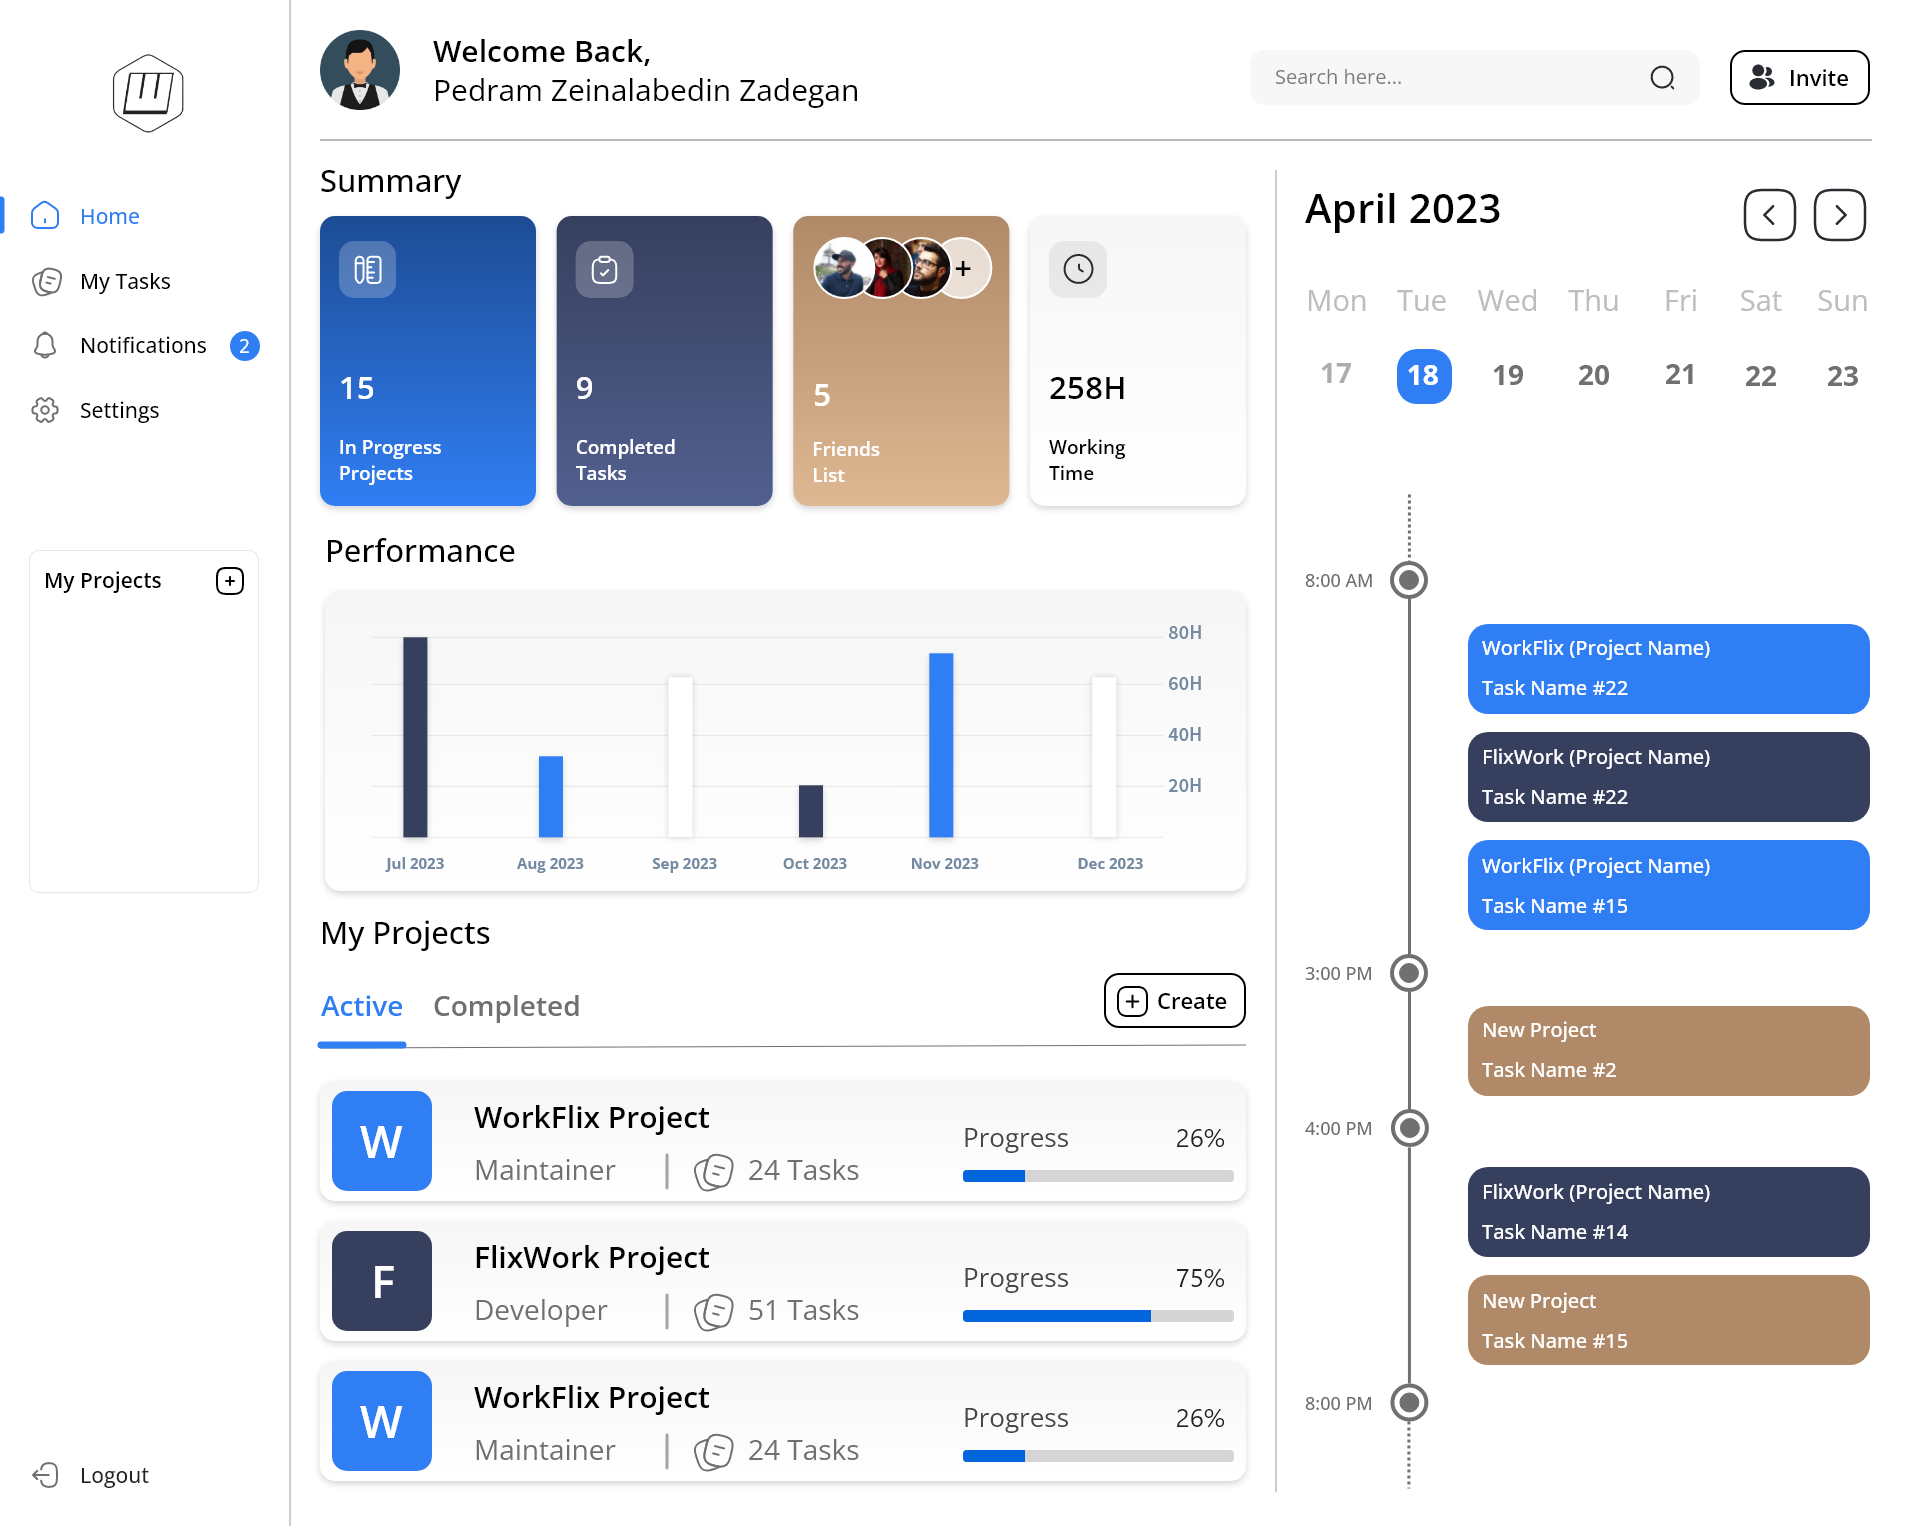
\includegraphics[width=\columnwidth]{images/Analytics.png}
